%% Appendix B — Parameter Adjustment Study Results
\chapter{Parameter Adjustment Study Results}
\label{app:prestudy_results}

The figures and tables below present the full ranking data from the five-round
parameter adjustment study described in \Cref{sec:prestudy_calibration}. Each bar
shows the percentage of participants who assigned a given option to that rank
position. Rows are sorted by Borda score. The Borda score for each option is the
sum of $(N - r)$ across all valid responses, where $N$ is the number of options
in that round and $r$ the rank position assigned by a participant. A higher Borda
score indicates a more consistently preferred option across the full distribution.
The mean rank (MR) is reported alongside; a lower value indicates higher preference.

\begin{figure}[H]
  \centering
  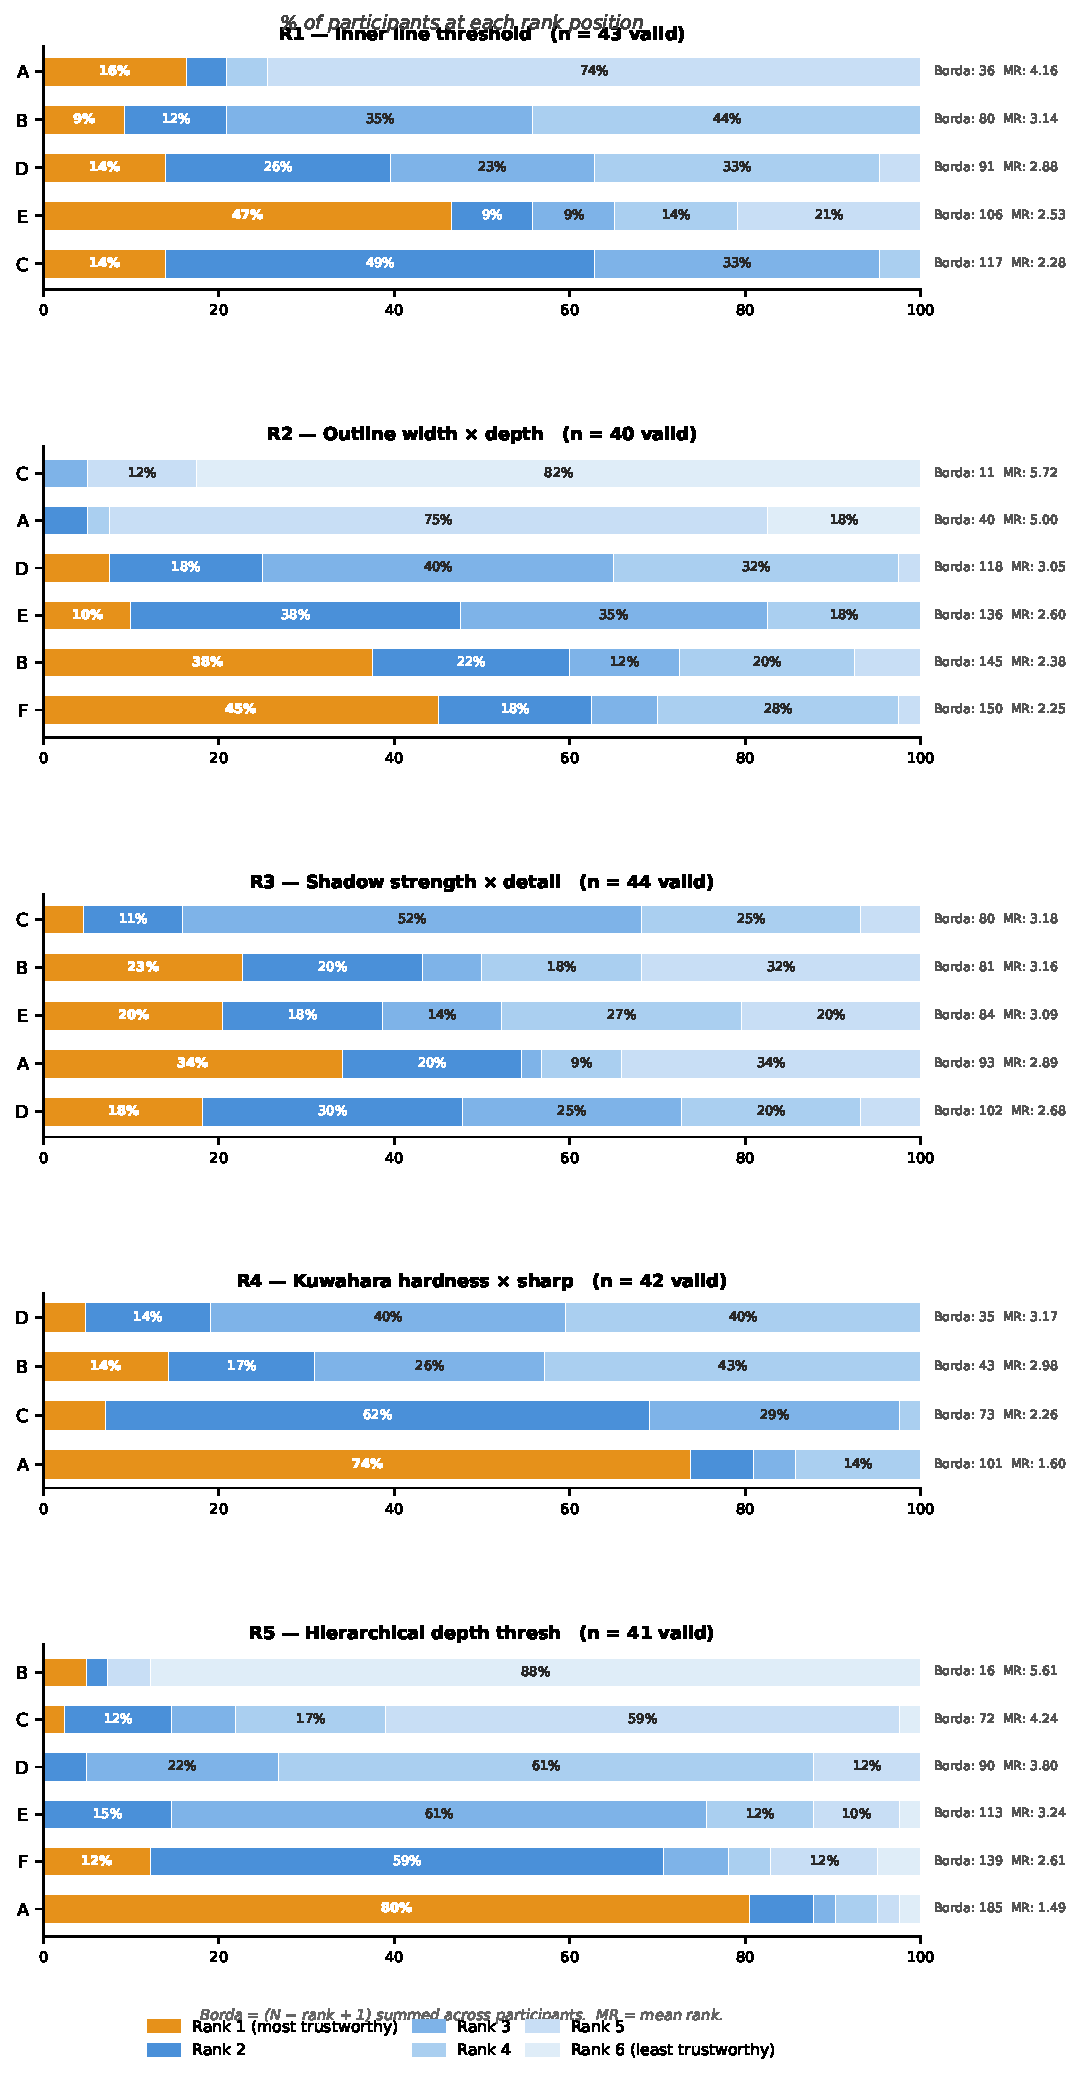
\includegraphics[width=\textwidth]{prestudy_round_results_full}
  \caption{Full rank distributions for all five parameter adjustment study rounds.
    Bars show the percentage of participants placing each option at each rank
    position; options within each round are sorted by Borda score (highest first).
    Borda and mean-rank (MR) annotations appear to the right of each bar.}
  \label{fig:prestudy_rounds}
\end{figure}

%%------------------------------------------------------------

The tables below list the computed Borda scores, maximum attainable score, mean
rank, and percentage ranked first for each option in each round. The winner by
Borda score is typeset in bold.

\bigskip
\noindent\textbf{Round 1 — Inner line threshold} \quad ($n = 43$ valid responses)

\smallskip
\begin{center}
\small
\begin{tabular}{lrrrr}
  \toprule
  Option & Borda & Max & Mean rank & \% ranked 1st \\
  \midrule
  \textbf{C} & 117 & 172 & 2.28 & 14.0\% \\
  E            & 106 & 172 & 2.53 & 46.5\% \\
  D            &  91 & 172 & 2.88 & 14.0\% \\
  B            &  80 & 172 & 3.14 &  9.3\% \\
  A            &  36 & 172 & 4.16 & 16.3\% \\
  \bottomrule
\end{tabular}
\end{center}

\bigskip
\noindent\textbf{Round 2 — Outline width $\times$ depth offset} \quad ($n = 40$ valid responses)

\smallskip
\begin{center}
\small
\begin{tabular}{lrrrr}
  \toprule
  Option & Borda & Max & Mean rank & \% ranked 1st \\
  \midrule
  \textbf{F} & 150 & 200 & 2.25 & 45.0\% \\
  B            & 145 & 200 & 2.38 & 37.5\% \\
  E            & 136 & 200 & 2.60 & 10.0\% \\
  D            & 118 & 200 & 3.05 &  7.5\% \\
  A            &  40 & 200 & 5.00 &  0.0\% \\
  C            &  11 & 200 & 5.72 &  0.0\% \\
  \bottomrule
\end{tabular}
\end{center}

\bigskip
\noindent\textbf{Round 3 — Shadow strength $\times$ detail bias} \quad ($n = 44$ valid responses)

\smallskip
\begin{center}
\small
\begin{tabular}{lrrrr}
  \toprule
  Option & Borda & Max & Mean rank & \% ranked 1st \\
  \midrule
  \textbf{D} & 102 & 176 & 2.68 & 18.2\% \\
  A            &  93 & 176 & 2.89 & 34.1\% \\
  E            &  84 & 176 & 3.09 & 20.5\% \\
  B            &  81 & 176 & 3.16 & 22.7\% \\
  C            &  80 & 176 & 3.18 &  4.5\% \\
  \bottomrule
\end{tabular}
\end{center}

\bigskip
\noindent\textbf{Round 4 — Kuwahara hardness $\times$ sharpness} \quad ($n = 42$ valid responses)

\smallskip
\begin{center}
\small
\begin{tabular}{lrrrr}
  \toprule
  Option & Borda & Max & Mean rank & \% ranked 1st \\
  \midrule
  \textbf{A} & 101 & 126 & 1.60 & 73.8\% \\
  C            &  73 & 126 & 2.26 &  7.1\% \\
  B            &  43 & 126 & 2.98 & 14.3\% \\
  D            &  35 & 126 & 3.17 &  4.8\% \\
  \bottomrule
\end{tabular}
\end{center}

\bigskip
\noindent\textbf{Round 5 — Hierarchical depth threshold} \quad ($n = 41$ valid responses)

\smallskip
\begin{center}
\small
\begin{tabular}{lrrrr}
  \toprule
  Option & Borda & Max & Mean rank & \% ranked 1st \\
  \midrule
  \textbf{A} & 185 & 205 & 1.49 & 80.5\% \\
  F            & 139 & 205 & 2.61 & 12.2\% \\
  E            & 113 & 205 & 3.24 &  0.0\% \\
  D            &  90 & 205 & 3.80 &  0.0\% \\
  C            &  72 & 205 & 4.24 &  2.4\% \\
  B            &  16 & 205 & 5.61 &  4.9\% \\
  \bottomrule
\end{tabular}
\end{center}

%%------------------------------------------------------------

\begin{figure}[H]
  \centering
  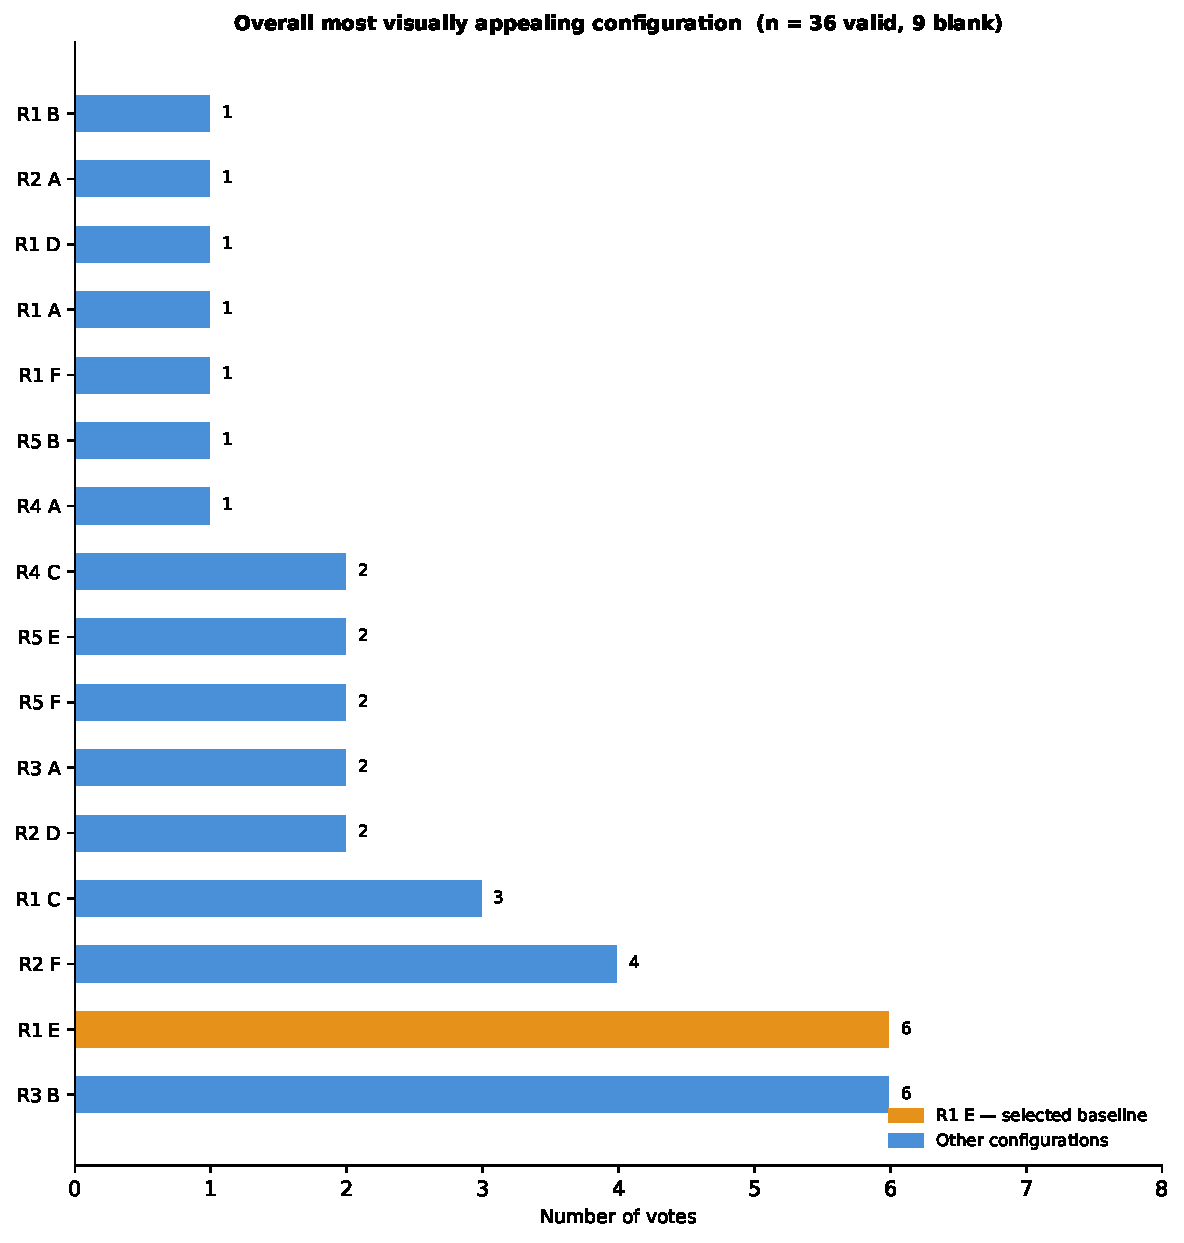
\includegraphics[width=0.85\textwidth]{prestudy_overall_appeal_full}
  \caption{Votes for the overall most visually appealing configuration from the
    final question of the parameter adjustment study ($n = 36$ valid, $9$ blank).
    The selected study baseline, R1\,E, is highlighted in amber.}
  \label{fig:prestudy_overall}
\end{figure}

\bigskip
\noindent\textbf{Overall visual appeal} \quad ($n = 36$ valid responses, $9$ blank)

\smallskip
\begin{center}
\small
\begin{tabular}{lr}
  \toprule
  Configuration & Votes \\
  \midrule
  R3\,B         & 6 \\
  \textbf{R1\,E} & 6 \\
  R2\,F         & 4 \\
  R1\,C         & 3 \\
  R2\,D         & 2 \\
  R3\,A         & 2 \\
  R5\,F         & 2 \\
  R5\,E         & 2 \\
  R4\,C         & 2 \\
  R4\,A         & 1 \\
  R5\,B         & 1 \\
  R1\,F         & 1 \\
  R1\,A         & 1 \\
  R1\,D         & 1 \\
  R2\,A         & 1 \\
  R1\,B         & 1 \\
  Blank         & 9 \\
  \bottomrule
\end{tabular}
\end{center}
